\section{Maximum Flow}
\tikzset{
  in place/.style={
    auto=false,
    fill=white,
    inner sep=2pt,
  },
}
  \tikzstyle{vertex}=[circle,fill=black!25,minimum size=20pt,inner sep=0pt]
  
  \tikzstyle{edge} = [draw,thick,-]
  \tikzstyle{diredge} = [draw,thick,->]
  \tikzstyle{selected diredge} = [draw,thick,->,red]

  \subsection{Motivation}
  \begin{frame}{Motivation}
  \setbeamercovered{invisible}
    

    \begin{figure}
        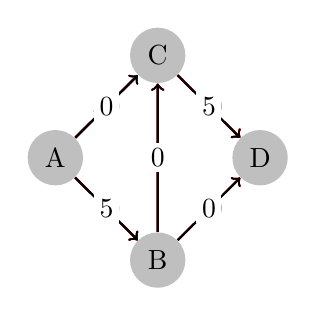
\begin{tikzpicture}[scale=1.3, auto,swap]
        \node[vertex] (A) at (0, 0) {A};
        \node[vertex] (B) at (1, -1) {B};
        \node[vertex] (C) at (1, 1) {C};
        \node[vertex] (D) at (2, 0) {D};
        
        \path[diredge]<1> (A) -- node[pos=0.5, in place] {70} (B);
        \path[diredge]<1-3> (A) -- node[pos=0.5, in place] {30} (C);
        \path[diredge]<1-3> (C) -- node[pos=0.5, in place] {50} (D);
        \path[diredge]<1> (B) -- node[pos=0.5, in place] {50} (D);
        \path[diredge]<1-4> (B) -- node[pos=0.5, in place] {15} (C);
      
      \path[selected diredge]<2> (A) -- node[pos=0.5, in place] {70} (B);
      \path[selected diredge]<2> (B) -- node[pos=0.5, in place] {50} (D);

      \path[diredge]<3-4> (A) -- node[pos=0.5, in place] {20} (B);
      \path[diredge]<3-6> (B) -- node[pos=0.5, in place] {0} (D);

      \path[selected diredge]<4> (A) -- node[pos=0.5, in place] {30} (C);
      \path[selected diredge]<4> (C) -- node[pos=0.5, in place] {50} (D);

      \path[diredge]<5-6> (A) -- node[pos=0.5, in place] {0} (C);
      \path[selected diredge]<5> (A) -- node[pos=0.5, in place] {20} (B);
      \path[selected diredge]<5> (B) -- node[pos=0.5, in place] {15} (C);
      \path[selected diredge]<5> (C) -- node[pos=0.5, in place] {20} (D);

      \path[diredge]<6> (A) -- node[pos=0.5, in place] {5} (B);
      \path[diredge]<6> (B) -- node[pos=0.5, in place] {0} (C);
      \path[diredge]<6> (C) -- node[pos=0.5, in place] {5} (D);
    
          
           
    \end{tikzpicture}
  \end{figure}
  \begin{center}
    \pause \pause 50
    \pause \pause  + 30
    \pause  + 15 = 95
  \end{center}

  
\end{frame}

\subsection{Ford Fulkerson}
\subsubsection{Algorithmus}
\begin{frame}{Ford Fulkerson}
  \setbeamercovered{invisible}
  %\rightarrow
  \begin{block}{Ford Fulkerson}
    \begin{itemize}
      \item mf = 0;
      \pause
      \item Solange ein Pfad p (s $\rightarrow$ ... i $\rightarrow$ j $\rightarrow$ ... $\rightarrow$ t) von source nach t existiert:
      \pause
      \begin{itemize}
      \item 1. finde minimale Kante f auf dem Pfad
      \pause
      \item 2. Kapazität aller Kanten in Pfadrichtung (z.B. i $\rightarrow$ j) um f reduzieren
      \pause
      \item 3. Kapazität aller Kanten gegen Pfadrichtung (z.B. j $\rightarrow$ i) um f erhöhen 
      \pause
      \item mf += f;
      \end{itemize}
    \end{itemize}
  \end{block}
\end{frame}
\subsubsection{Rückkante}
\begin{frame}{Rückkante}
  \setbeamercovered{invisible}
  \begin{figure}
    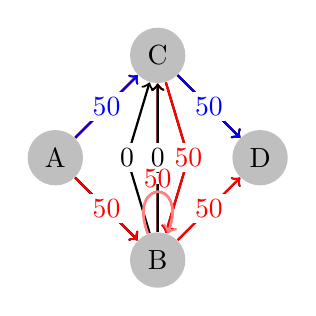
\begin{tikzpicture}[scale=1.3, auto,swap]
    \node[vertex] (A) at (0, 0) {A};
    \node[vertex] (B) at (1, -1) {B};
    \node[vertex] (C) at (1, 1) {C};
    \node[vertex] (D) at (2, 0) {D};
    
    \path[diredge]<1> (A) -- node[pos=0.5, in place] {50} (B);
    \path[diredge]<1-4> (A) -- node[pos=0.5, in place] {50} (C);
    \path[diredge]<1> (C) -- node[pos=0.5, in place] {50} (D);
    \path[diredge]<1-4> (B) -- node[pos=0.5, in place] {50} (D);
    \path[diredge]<1> (B) -- node[pos=0.5, in place] {50} (C);
      
    \path[selected diredge]<2> (A) -- node[pos=0.5, in place] {50} (B);
    \path[selected diredge]<2> (B) -- node[pos=0.5, in place] {50} (C);
    \path[selected diredge]<2> (C) -- node[pos=0.5, in place] {50} (D);
      
    \path[diredge]<3-5> (A) -- node[pos=0.5, in place] {0} (B);
    \path[diredge]<3-5> (C) -- node[pos=0.5, in place] {0} (D);
    \path[diredge]<3> (B) -- node[pos=0.5, in place] {0} (C);
      
    \path[diredge]<4-5> (B) -- (0.7,0);
    \path[diredge]<4-5> (0.7, 0) -- node[pos=0, in place] {0} (C);
    \path[diredge]<4> (1.3,0) -- (B) ;
    \path[diredge]<4> (C) -- node[pos=1, in place] {50} (1.3,0);

    \path[selected diredge]<5> (1.3,0) -- (B) ;
    \path[selected diredge]<5> (C) -- node[pos=1, in place] {50} (1.3,0);
    
    

      %\node[] (M) at (1.3, 0) [label=center:\textcolor{red}{$50$}];
    \path[selected diredge]<5> (A) -- node[pos=0.5, in place] {50} (C);
    \path[selected diredge]<5-6> (B) -- node[pos=0.5, in place] {50} (D);
    \pause    
    \pause    
    \pause    
    \pause    
    \pause    
    % Auskommentiert damit das Kompilieren Fehlerfrei läuft --> Vor Präsi wegnehmen !!
    \node[in place] (T) at (1,-0.2) [label=center:\color{red}{$50$}] {};
    \draw[line width= 1pt,->, red!50] (B) .. controls (0.7, -0.2) and (1.3, -0.2) .. (B); 
    \path[selected diredge]<6> (A) -- node[pos=0.5, in place] {50} (B);  
    \path[draw,thick,->,blue]<6> (C) -- node[pos=0.5, in place] {50} (D);  
    \path[draw,thick,->,blue]<6> (A) -- node[pos=0.5, in place] {50} (C);
    
    
    \end{tikzpicture}
  \end{figure}
\end{frame}
\subsubsection{Laufzeit}
\begin{frame}{Laufzeit}
  \setbeamercovered{invisible}
  \begin{block}{Laufzeit Ford Fulkerson}
      \begin{itemize}
        \item O(ES)
        \pause
        \item wobei S die Lösung ist
        \pause
        \item O(S) mal Tiefensuche, was in O(E) läuft, da $E \geq$ V - 1
      \end{itemize}
      \pause
      $\Rightarrow$ kann sehr groß werden
  \end{block}
\end{frame}
\begin{frame}{Laufzeit Beispiel}
  \setbeamercovered{invisible}
  \begin{figure}
    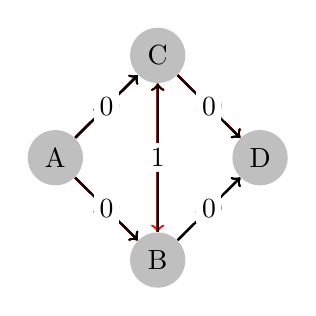
\begin{tikzpicture}[scale=1.3, auto,swap]
    \node[vertex] (A) at (0, 0) {A};
    \node[vertex] (B) at (1, -1) {B};
    \node[vertex] (C) at (1, 1) {C};
    \node[vertex] (D) at (2, 0) {D};
    
    \path[diredge]<1> (A) -- node[pos=0.5, in place] {50} (B);
    \path[diredge]<1-2> (A) -- node[pos=0.5, in place] {50} (C);
    \path[diredge]<1> (C) -- node[pos=0.5, in place] {50} (D);
    \path[diredge]<1-2> (B) -- node[pos=0.5, in place] {50} (D);
    \path[diredge]<1> (B) -- node[pos=0.5, in place] {1} (C);
    
    \path[selected diredge]<2> (A) -- node[pos=0.5, in place] {50} (B);
    \path[selected diredge]<2> (B) -- node[pos=0.5, in place] {1} (C);
    \path[selected diredge]<2> (C) -- node[pos=0.5, in place] {50} (D);
      
    \path[diredge]<3> (A) -- node[pos=0.5, in place] {49} (B);
    \path[diredge]<3> (C) -- node[pos=0.5, in place] {49} (D);
    \path[selected diredge]<3> (C) -- node[pos=0.5, in place] {1} (B);
    \path[selected diredge]<3> (A) -- node[pos=0.5, in place] {50} (C);
    \path[selected diredge]<3> (B) -- node[pos=0.5, in place] {50} (D);

    \path[selected diredge]<4> (A) -- node[pos=0.5, in place] {49} (B);
    \path[selected diredge]<4> (B) -- node[pos=0.5, in place] {1} (C);
    \path[selected diredge]<4> (C) -- node[pos=0.5, in place] {49} (D);
    \path[diredge]<4> (A) -- node[pos=0.5, in place] {49} (C);
    \path[diredge]<4> (B) -- node[pos=0.5, in place] {49} (D);

    \path[diredge]<5> (A) -- node[pos=0.5, in place] {0} (B);
    \path[diredge]<5> (A) -- node[pos=0.5, in place] {0} (C);
    \path[diredge]<5> (C) -- node[pos=0.5, in place] {0} (D);
    \path[diredge]<5> (B) -- node[pos=0.5, in place] {0} (D);
    \path[diredge]<5> (B) -- node[pos=0.5, in place] {1} (C);

    \end{tikzpicture}
  \end{figure}
  

\end{frame}
\subsection{Edmond Karp}
\begin{frame}{Edmond Karp}
  \setbeamercovered{invisible}
  \begin{block}{Unterschied zu Ford Fulkerson}
    \begin{itemize}
      \item Breitensuche statt Tiefensuche
      \pause
      \item Laufzeit O(V$E^2$)
      \pause
      \item O(VE) mal Breitensuche, was in O(E) läuft
    \end{itemize}
  \end{block}
\end{frame}